\subsubsection{Visualizar Solicitud}
En la siguiente figura \ref{fig:Diagrama de Secuencia - Visualizar Solicitudes de Refaccion} se muestra el diagrama de secuencia que corresponde a la visualización de todas las solicitudes que los diversos empleados han realizado para que puedan hacer su trabajo, existen dos posibilidades dentro de esta actividad:
\begin{itemize}
	\item \textbf{Si existen registros:} Al momento de que el administrador entra a esta parte del sistema, se muestra en una tabla y/o lista toda la información necesaria para atender a las solicitudes que se necesiten.  
	\item \textbf{No existen registros:} No hay empleados registrados, se muestra una tabla y/o lista vacía en pantalla.
\end{itemize}
\begin{figure}[!h]
	\centering
	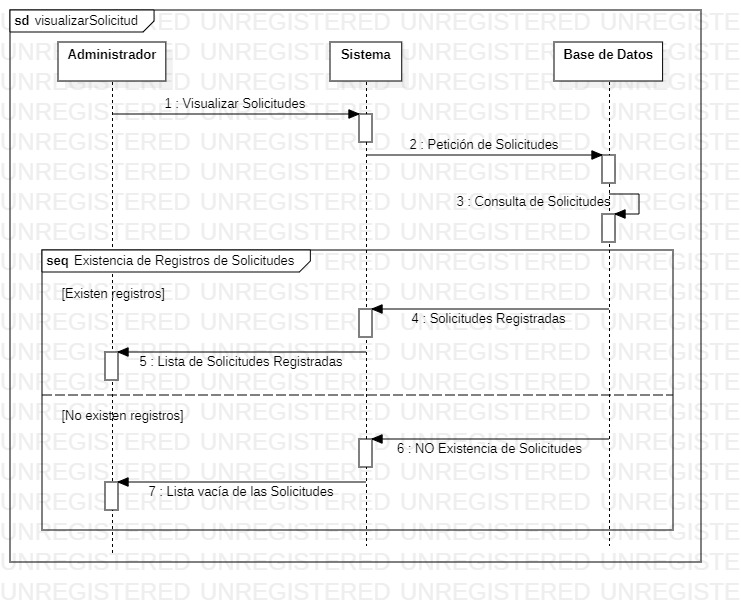
\includegraphics[width=0.8\textwidth]{./diseno/vprocesos/imagenes/visualizarSolicitud}
	\caption{Diagrama de Secuencia - Visualizar Solicitudes de Refacción}
	\label{fig:Diagrama de Secuencia - Visualizar Solicitudes de Refaccion}
\end{figure}
\clearpage